In questo capitolo verrà affrontata la generazione del grafo di scena dato un frame e l'aggiornamento della Mappa Semantica con queste nuove informazioni per manterla aggiornata rispetto all'ambiente.
\begin{figure}[h]
  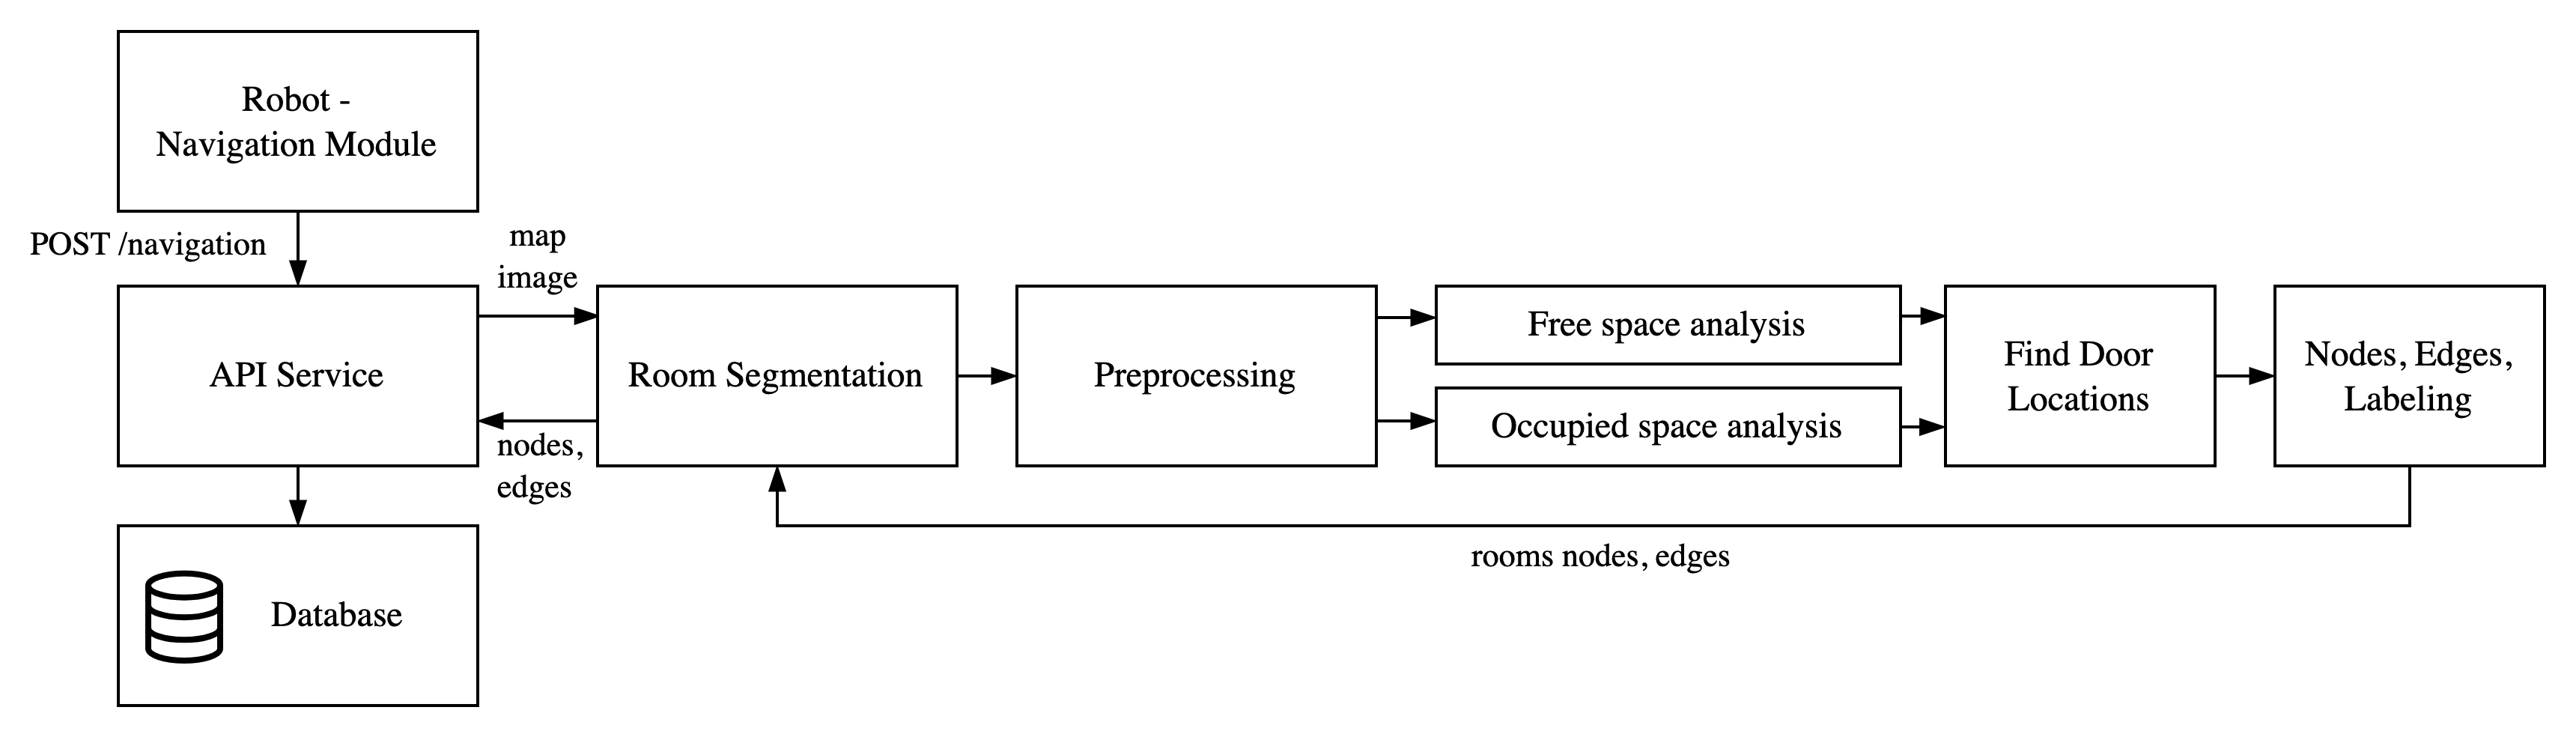
\includegraphics[width=\textwidth]{scene_graph/general_data_flow.png}
  \caption{Schema dei flussi dati per la generazione del grafo di scena e aggiornamento della mappa semantica }
\end{figure}

\section{Generazione del Grafo di Scena}
La generazione del grafo di scena è un passo fondamentale per il mantenimento della coerenza tra Mappa Semantica e Ambiente reale.\\
Il grafo di scena è una struttura dati che rappresenta gli oggetti presenti nell'ambiente e le relazioni tra loro composto da nodi e archi. I nodi rappresentano gli oggetti, mentre gli archi rappresentano le relazioni tra gli oggetti.

\subsection{Lettura del frame RGB-D}
All'interno dell'architettura cloud-native di Robee vi è la presenza di un pod chiamato "Streaming Module" il cui compito è streammare il feed video delle camera sul pod redis del robot, in modo che gli altri servizi o moduli possano accedere a questi dati tramite l'utilizzo di librerie wrapper, rendendo il tutto agnostico rispetto alla tipologia e modello di videocamera montati.

\subsection{Inferenza}
Ogni frame ricevuto dal feed video viene successivamente dato in input al modello PSGTr \cite{yang2022psg} che restituisce un oggetto di tipo Detections il quale contiene i seguenti dati:
\begin{itemize}
  \item labels: lista con lunghezza pari al numero di oggetti rilevati. Ogni valore indica la label corrispondente all' $i$-esimo oggetto. Per esempio, l'oggetto $i$-esimo ha label $labels[i]$;
  \item masks: lista contenente le maschere di ogni oggetto rilevato;
  \item bboxes: lista contenente le bounding boxes di ogni oggetto rilevato;
  \item rel\_pair\_idxes: lista con lunghezza pari al numero di relazioni tra oggetti rilevate. Ogni valore è a sua volta un array di dimensione due dove il primo elemento è l'oggetto target della relazione e il secondo è l'oggetto sorgente della relazione;
  \item rel\_labels: lista con lunghezza pari al numero di relazioni tra oggetti rilevate. Ogni valore indica la label della $i$-esima relazione
  \item rel\_dists: lista con lunghezza pari al numero di relazione tra oggetti rilevate. Ogni valore indica la probabilità associata alla $i$-esima relazione.
\end{itemize}
Questi dati vengono successivamente utilizzati per la costruzione del grafo di scena mediante l'algoritmo seguente.

\subsubsection{Panoptic Scene Graph - Transformer}
Il modello PSGTr \cite{yang2022psg} è un modello di deep learning a singolo stato basato su architettura Transformer \cite{transformer} il cui obiettivo è quello di generare una rappresentazione a grafo della scena data la segmentazione panottica piuttosto che le bounding box degli oggetti rilevati.
\paragraph*{Training}
Il modello, per quanto riguarda gli oggetti, è stato addestrato su un dataset composto da 49mila immagini annotate basato su COCO \cite{coco} e Visual Genome \cite{visualgenemo}. Per le relazioni hanno estratto e costruito un dataset di 56 predicati a partire da dataset come VG-150 \cite{vg150}, VrR-VG \cite{vrvvg} and GQA \cite{cqa}.
\paragraph*{Segmentazione Panoptica}
La segmentazione panoptica individua gli oggetti e assegna a ogni pixel la label della classe dell'oggetto a cui appartengono. L'utilizzo di questa rispetto alle bounding da notevoli vantaggi:
\begin{itemize}
  \item Garantisce una localizzazione più precisa degli oggetti, segmentandoli a livello di pixel e riducendo la presenza di pixel rumorosi o ambigui tipici delle bounding box, che spesso includono porzioni di altre categorie o oggetti;
  \item Copre l'intera scena di un'immagine, inclusi gli sfondi, offrendo una comprensione più completa del contesto rispetto alle bounding box, che tendono a trascurare importanti informazioni di sfondo;
  \item Riduce anche le informazioni ridondanti o irrilevanti presenti nei dataset basati su bounding box, focalizzandosi sulla segmentazione degli oggetti piuttosto che sulle loro parti.
\end{itemize}
\paragraph*{Funzionamento di PSGTr}
L'architettura di PSGTr è basata su DETR \cite{detr} e HOI \cite{hoi}. Il modello predice triple $(soggetto, predicato, verbo)$ e la localizzazione degli oggetti simultaneamente.
\subparagraph*{Pipeline PSGTr}
Attraverso una \gls{backbone} CNN, PSGTr estrae le features dell'immagine e i positional encodings che, insieme alle triplet queries, vengono dati in input al transformer encoder-decoder. In questo processo, l'obiettivo è che le query apprendano la rappresentazione del grafo di scena a triple in modo che per ognuna di esse, le predictions di  $(soggetto, predicato, verbo)$ possano successivamente essere estratte da tre Feed Forward Network. Infine, il task di segmentazione viene eseguito da due head panoptiche, una per il soggetto e una per l'oggetto della relazione.

\subsection{Costruzione del grafo}
L'obiettivo di questo step è la costruzione del grafo di scena rispetto all'ultimo frame. Per farlo, è necessario estrarre i dati dai risultati dell'inferenza di PSGTr e calcolare quei valori che dipendono dal sistema robot, come la posizione. 
L'algoritmo di costruzione del grafo è costituito da 2 fasi principali:
\begin{itemize}
  \item Costruzione dei nodi per la scena semantica e per la mappa semantica:
  \begin{itemize}
    \item Calcolo della posizione dell'oggetto
  \end{itemize}
  \item Costruzione degli archi per la scena semantica e per la mappa semantica
\end{itemize}

\subsubsection{Costruzione dei nodi}
\paragraph{Estrazione dati dai risultati}
L'oggetto MMDetResult ritornato dalla funzione di inferenza del modello, come detto precedentemente, possiede un attributo $labels$ che è una lista con lunghezza pari al numero di oggetti rilevati dove il valore $i$-esimo, indica l'indice della classe di appartenenza dell'oggetto $i$. Lo stesso meccanismo vale anche per le maschere.

\begin{algorithm}
  \caption{Estrazione classi e maschere degli oggetti individuati}
  \begin{algorithmic}[1]
    \State $obj\_classes \gets \text{[ ]}$
    \State $obj\_masks \gets \text{[ ]}$
    \State $obj\_labels\_ids \gets detectionResults.labels$
    \For{ $i=0$ to $obj\_labels\_ids.length$}
      \State $obj\_classes.append(PSG\_CLASSES[obj\_labels\_ids[i]])$
      \State $obj\_masks.append(detectionResults.masks[i])$
    \EndFor
  \end{algorithmic}
\end{algorithm}


\paragraph{Calcolo posizioni 3d}
Per ogni oggetto, si estrae la posizione 3D nella mappa del robot in modo che questo possa successivamente localizzarlo e raggiungerlo.
\subparagraph{Utilizzo del Point Cloud}
\subparagraph{Utilizzo della Matrice Inversa della Camera}
\subparagraph{Utilizzo della Matrici di trasformazione}

\subsubsection{Costruzione degli archi}

\section{Aggiormento del Mappa Semantica}
\subsection{Stanza corrente robot}
\subsection{Proiezione del Camera Frustum}
\subsection{Controllo della posizione degli oggetti}
\subsection{Aggiornamento e salvataggio a DB}



\section{Conclusioni}

